\documentclass[10pt, compress, aspectratio=169]{beamer}

% DZ: My MikTeX freezes when trying to compile the source with the metropolis theme.
%\usetheme{metropolis}
\usepackage{appendixnumberbeamer}

\usepackage{tikz-dependency}
\usepackage{caption}
\usepackage{booktabs}
\usepackage{fontspec}
\usepackage[scale=2]{ccicons}

\usepackage{pgfplots}
\usepgfplotslibrary{dateplot}

\usepackage{xspace}

%\setmainfont[Script=Devanagari]{FreeSans}
\newfontfamily\devnag[Script=Devanagari]{Lohit Devanagari}
\newfontfamily\cyrl[Script=Cyrillic]{FreeSans}

\newcommand{\themename}{\textbf{\textsc{metropolis}}\xspace}

% commands from the paper
\newfontfamily\gtfont[Scale=1.1,Letters=SmallCaps]{Linux Libertine O}
\newcommand{\udtag}[1]{{\ll \textsc{#1}}}
\newcommand{\gtlabel}[1]{{\gtfont #1}}
\newcommand{\udlabel}[1]{{\tt #1}}
\newfontfamily\udfont[Scale=0.9,Letters=SmallCaps]{Linux Libertine O}
\newcommand{\utag}[1]{{\udfont#1}}
\newcommand{\ufeat}[1]{{\udfont#1}}
\newcommand{\tgl}[1]{{\em #1}}
% commands from the paper

\newcommand{\grey}[1]{\textcolor{lightgray}{#1}}

\setbeamertemplate{navigation symbols}{}
\setbeamertemplate{footline}{
  \hfill%
  \usebeamercolor[fg]{page number in head/foot}%
  \usebeamerfont{page number in head/foot}%
  \setbeamertemplate{page number in head/foot}[framenumber]%
  \usebeamertemplate*{page number in head/foot}\kern3.5em\vskip10pt%
}


\title{Tutorial on Universal Dependencies\\
{\small Cross-linguistically consistent syntactic annotation}}
\date{\today}
\date{}
\author{%
\textbf{Marie-Catherine de Marneffe}\inst{1}
\and
Joakim Nivre\inst{2}
\and
Daniel Zeman\inst{3}
\vspace{0.5cm}
}
\institute[shortinst]{%
\inst{1}
FNRS,
Université catholique de Louvain, Belgium
\and
\inst{2}
Department of Linguistics and Philology,
Uppsala University, Sweden
\and
\inst{3}
Institute of Formal and Applied Linguistics,
Charles University, Prague, Czechia
}
\logo{\hfill
\includegraphics[height=1.25cm]{images/ud-logo-transp.png}}


\begin{document}

\maketitle

%\begin{frame}{Table of contents}
%  \setbeamertemplate{section in toc}[sections numbered]
%  \tableofcontents[hideallsubsections]
%
%\begin{itemize}
%  \item Basic clauses
%  \item Nominal phrases
%  \item Complex clauses
%  \item Ellipsis
%\end{itemize}
%
%\end{frame}

\begin{frame}
\frametitle{Cross-lingual Syntax}

% Idea: Go through the structures we expect to find in all languages and explain how they are dealt with in UD

How can we do cross-lingual syntax ?

\begin{itemize}
  \item Find the structures we expect to find in all languages
  \item Describe how they are dealt with
  \begin{itemize}
    \item Using a representation that facilitates cross-linguistic parallelism
  \end{itemize}
  \item Allow language-specific extensions
\end{itemize}

\end{frame}

\begin{frame}
  \frametitle{Approaches}
 % Other systems/frameworks: cross-linguality * -> english
 % UD: cross-linguality * <-> *

\begin{center}
\begin{columns}
\column{0.5\textwidth}
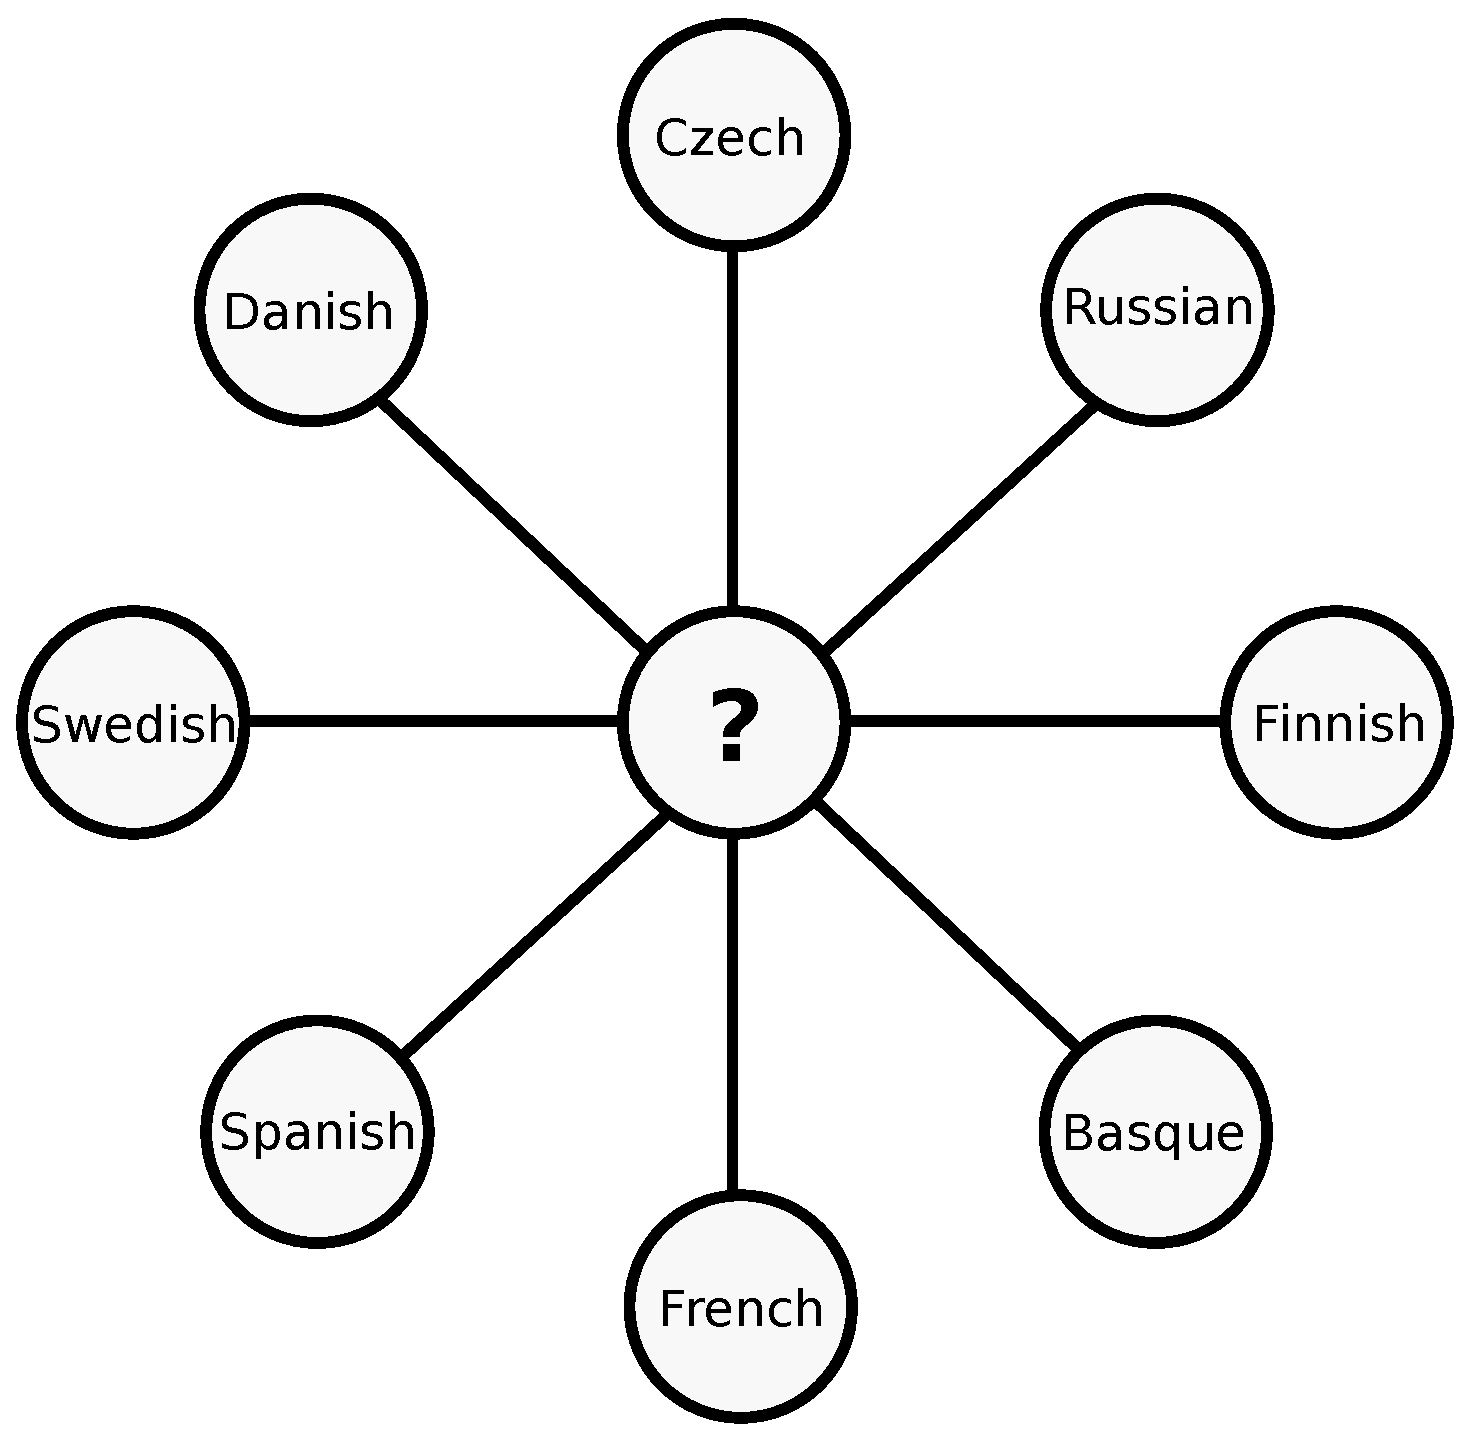
\includegraphics[width=0.8\textwidth]{images/other-interlingua.eps}

\column{0.5\textwidth}
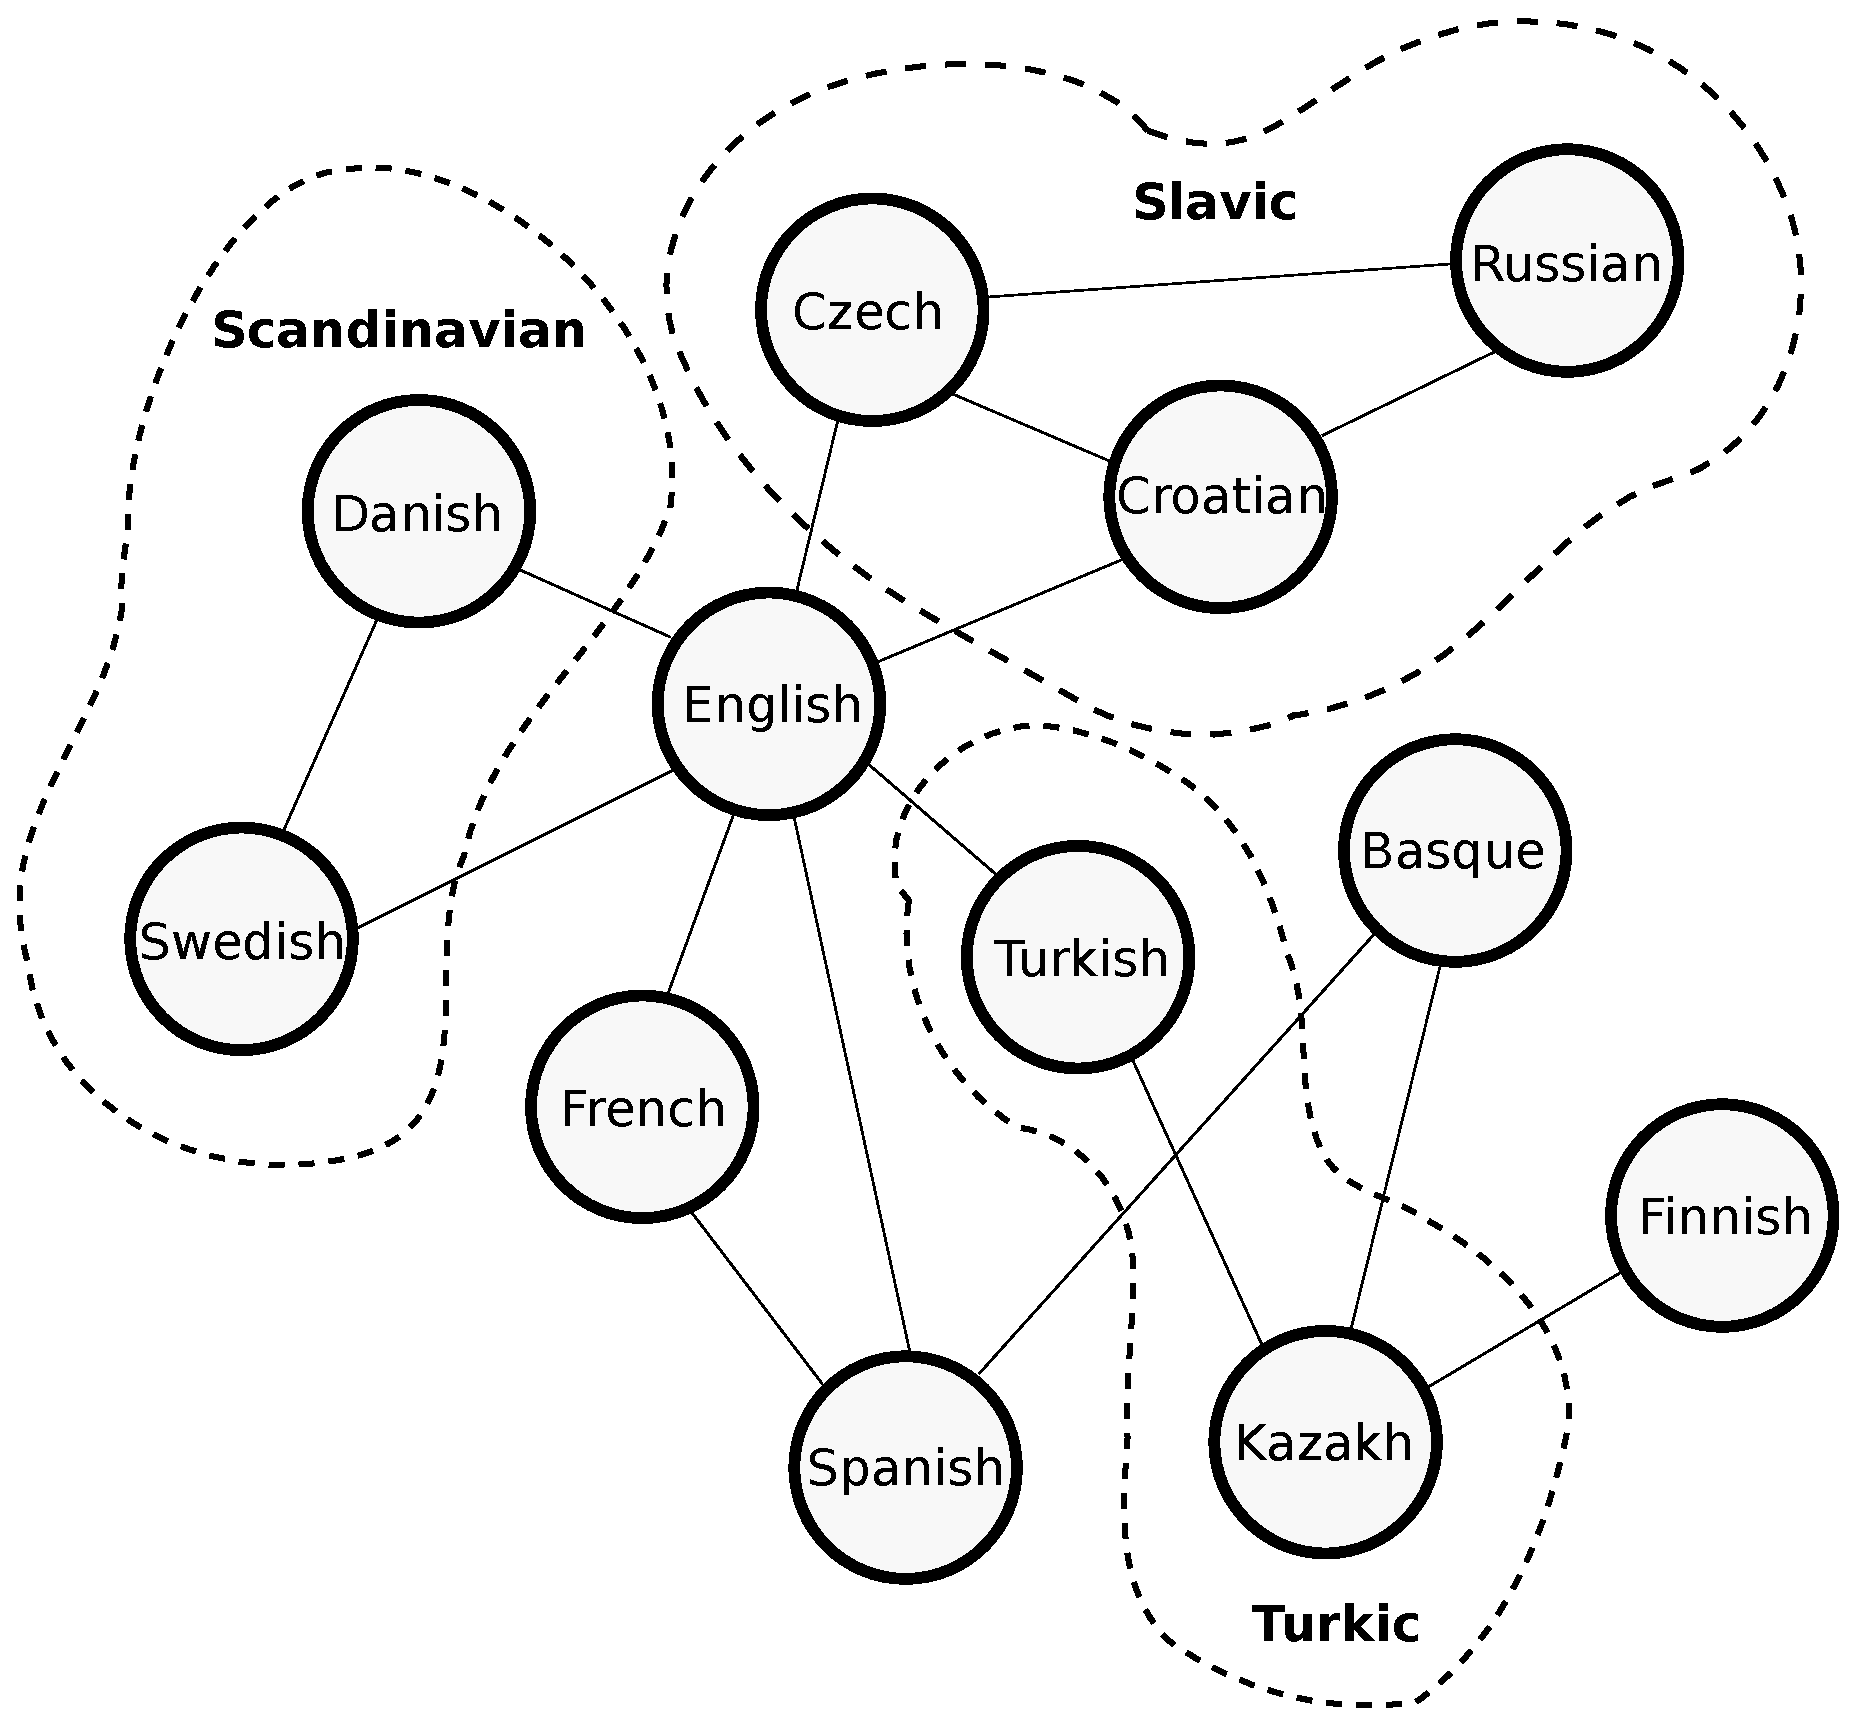
\includegraphics[width=0.85\textwidth]{images/ud-interlingua.eps}

\end{columns}

\end{center}
UD tries to standardise between languages, and particularly:
\begin{itemize}
  \item Within language groups
  \item Between typologically similar constructions
\end{itemize}

\end{frame}

% 30 mins = 20-30 slides

% Constructions, strategies, representations

% Problem with |----| grammaticalisation

%   - Basic clauses (intransitive, transitive, nominal)



\begin{frame}{Syntactic Annotation in UD}
\begin{itemize}
\item  Basic principles:
\begin{itemize}
\item  The primacy of content words
\item  Clauses, nominals and modifier words
\item  Core arguments vs.\ oblique dependents
\end{itemize}
\item  Universal and language-specific relations
\item  Basic and enhanced dependencies
\end{itemize}
\end{frame}

\begin{frame}{The Primacy of Content Words}

\centering
\bigskip
\scalebox{0.75}{
en: 
\begin{dependency}[label style={thick, font=\bfseries}]
\begin{deptext}[column sep=3pt, font=\bfseries]
The \& dog \& was \&[12pt] chased \& by \& the \& cat \\[0.1cm]
DET \& NOUN \& AUX \& VERB \& ADP \& DET \& NOUN \\
\end{deptext}
\depedge[edge style=red, thick]{2}{1}{det}
\depedge[edge style=blue, thick]{4}{2}{nsubj:pass}
\depedge[edge style=red, thick]{4}{3}{aux:pass}
%\deproot[edge style=blue, thick, edge unit distance=3ex]{4}{root}
\depedge[edge style=red, thick, edge unit distance=1.8ex]{7}{5}{case}
\depedge[edge style=red, thick, edge unit distance=1ex]{7}{6}{det}
\depedge[edge style=blue, thick, edge unit distance=2.1ex]{4}{7}{obl}
%\depedge[edge style=thick, edge unit distance=3ex]{4}{8}{punct}
\end{dependency}
}

\smallskip
\scalebox{0.75}{
sv: 
\begin{dependency}[label style={thick, font=\bfseries}]
\begin{deptext}[column sep=5pt, font=\bfseries]
\&[6pt] Hunden \&[16pt] jagades \&[0pt] av \& katten \& \\[0.1cm]
\& NOUN \& VERB \&[0pt] ADP \& NOUN \& \\[0.1cm]

\& \textcolor{red}{Definite=Def}  \& \textcolor{red}{Voice=Pass} \&[0pt] \& \textcolor{red}{Definite=Def} \& \\
\end{deptext}
\depedge[edge style=blue, thick, edge unit distance=5.8ex]{3}{2}{nsubj:pass}
%\deproot[edge style=blue, thick, edge unit distance=3ex]{3}{root}
\depedge[edge style=red, thick]{5}{4}{case}
\depedge[edge style=blue, thick]{3}{5}{obl}
%\depedge[edge style=thick, edge unit distance=3ex]{2}{5}{punct}
\end{dependency}
}

\smallskip
\scalebox{0.75}{
cs: 
\begin{dependency}[label style={thick, font=\bfseries}]
\begin{deptext}[column sep=5pt, font=\bfseries]
\&[18pt] Pes \& byl \&hon\v{e}n \&[45pt] ko\v{c}kou \\[0.1cm]
\& NOUN \&[0pt] AUX \& VERB \& NOUN \\[0.1cm]
\& \&  \& \textcolor{red}{Voice=Pass}\& \textcolor{red}{Case=Ins} \& \\
\end{deptext}
\depedge[edge style=blue, thick]{4}{2}{nsubj:pass}
%\deproot[edge style=blue, thick, edge unit distance=3ex]{4}{root}
\depedge[edge style=red, thick, edge start x offset=-3pt]{4}{3}{aux:pass}
%\depedge[edge style=red, thick]{4}{3}{case}
\depedge[edge style=blue, thick, edge unit distance=6ex]{4}{5}{obl}
%\depedge[edge style=thick, edge unit distance=3ex]{2}{5}{punct}
\end{dependency}
}

\end{frame}

\begin{frame}{Three Types of Structures}
\begin{tabular}{cccc}
\textcolor{orange}{The dog} & chased & \textcolor{orange}{the cat} & \textcolor{blue}{from the room}\\
& & & \\
\textcolor{orange}{entity}  & event & \textcolor{orange}{entity} & \textcolor{blue}{attribute}\\
& & & \\
NOMINAL & CLAUSE & NOMINAL & MODIFIER\\
\end{tabular}

\end{frame}

\begin{frame}{Core Arguments}
\begin{itemize}
\item Arguments of basic intransitive and transitive verbs
\item Distinguished by one or more of the following properties:
\begin{itemize}
\item Verbs usually only agree with core arguments
\item Core arguments normally appear without adpositions
\item Certain cases, traditionally called nominative, accusative, and absolutive are typically reserved core arguments
\item Core arguments often occupy special positions in the clause
\item Syntactic phenomena like control, relativisation and passivisation can be restricted to core arguments
\end{itemize}
\item UD distinguishes core arguments from oblique dependents
\item UD does \textcolor{red}{not} distinguish arguments from adjuncts
\end{itemize}
\end{frame}


\begin{frame}{Syntactic Relations}
\centering
\bigskip
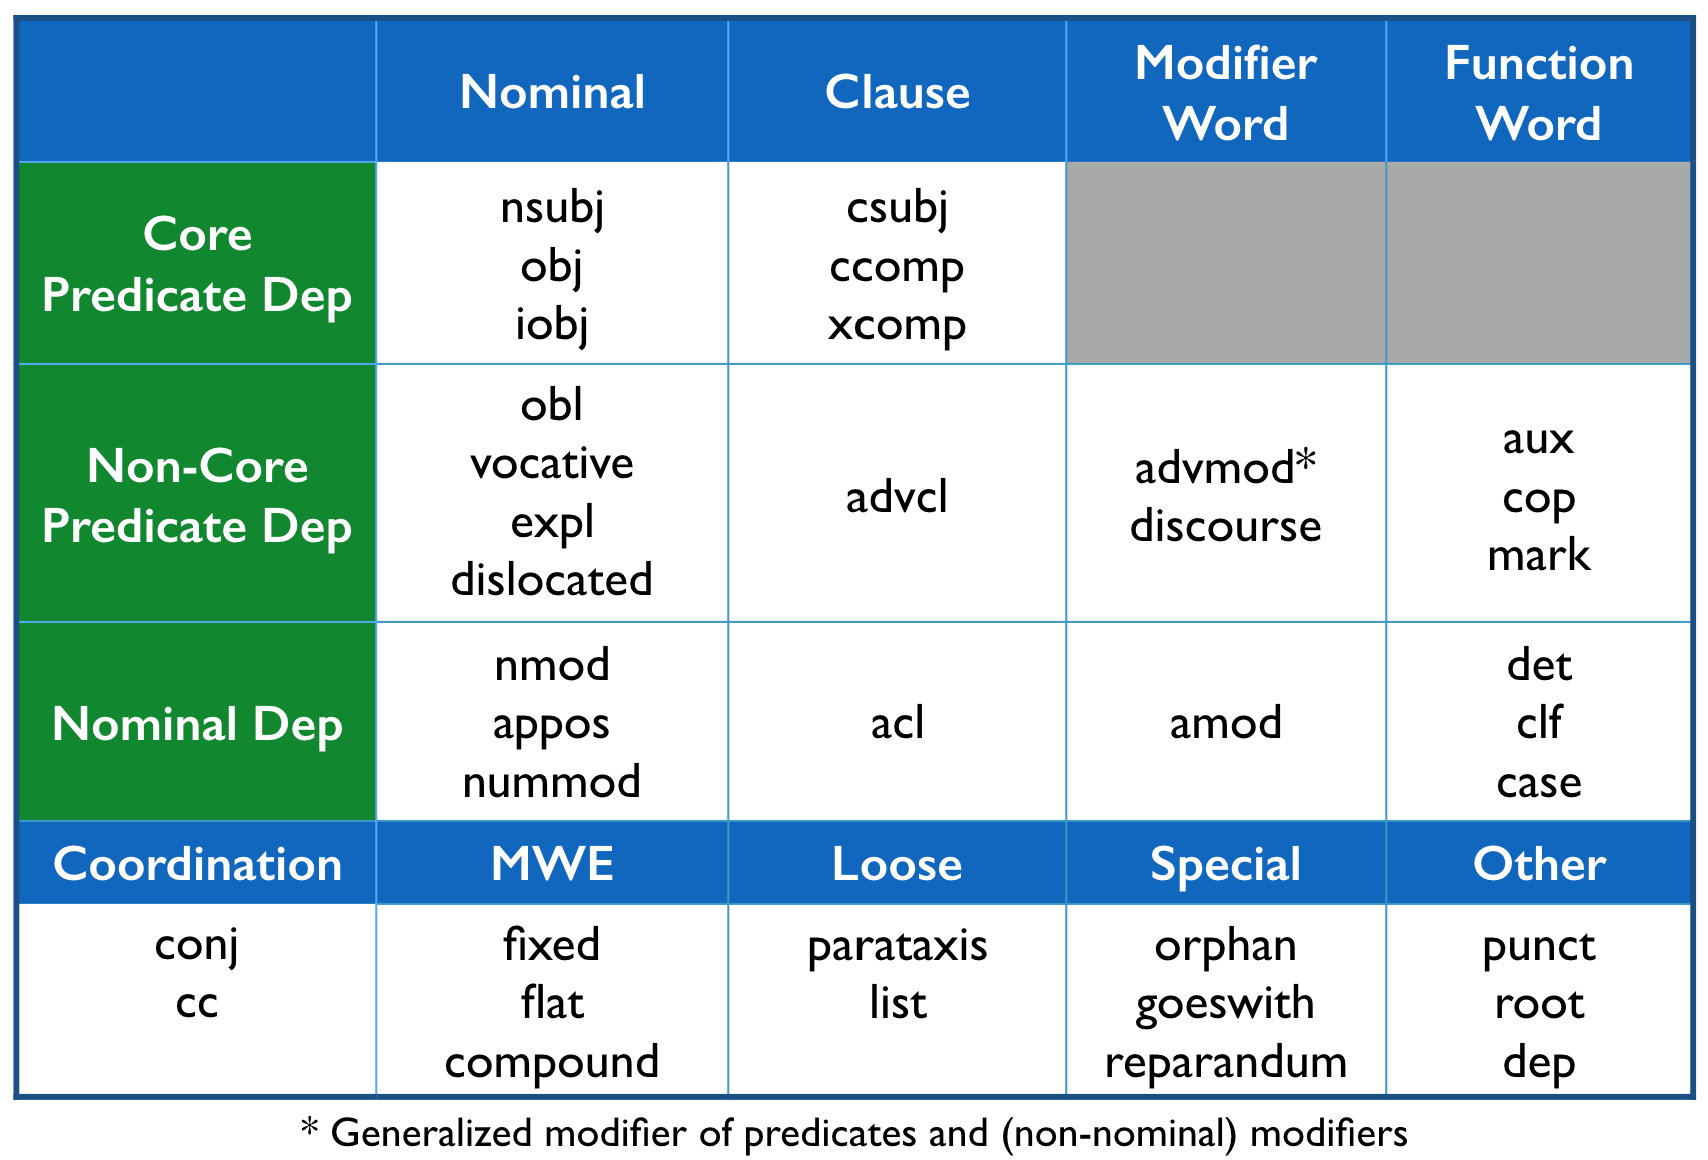
\includegraphics[scale=0.33]{images/taxonomy.png}
\end{frame}


\begin{frame}{A Two-Level Architecture}
\begin{itemize}
\item Universal relations
\begin{itemize}
\item Broad categories to allow cross-linguistic comparison
\end{itemize}
\item Language-specific relations
\begin{itemize}
\item Subtypes to capture language-specific phenomena
\end{itemize}
\end{itemize}

\centering
\bigskip
\begin{tabular}{|c|c|}
\hline
\textbf{Universal} & \textbf{Language-Specific} \\
\hline
acl & acl:relcl \\
compound & compound:prt \\
nmod & nmod:poss \\
\hline
\end{tabular}

%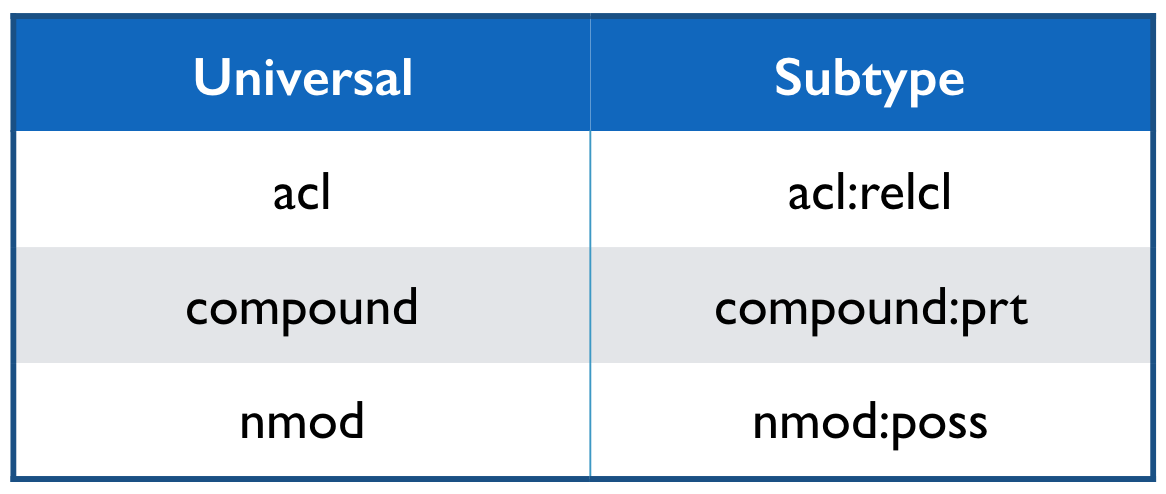
\includegraphics[scale=0.33]{subtypes}
\end{frame}


\begin{frame}
 \frametitle{Clauses}

\vspace{0.5cm}
\begin{columns}

\column{0.5\textwidth}
\begin{center}
  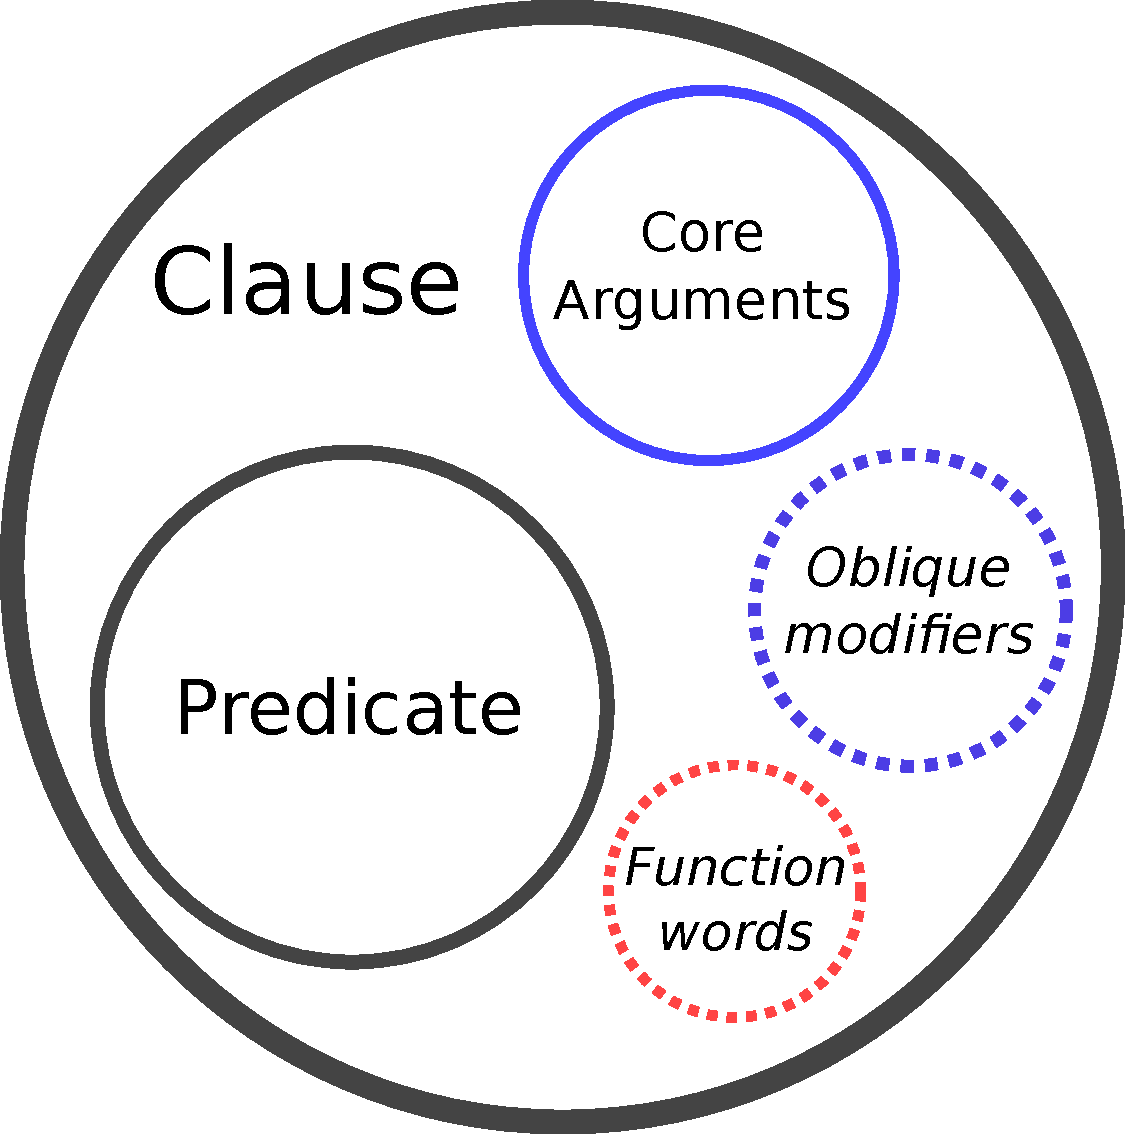
\includegraphics[width=0.5\textwidth]{images/clause.pdf}
\end{center}

\column{0.5\textwidth}
\begin{center}
\scalebox{0.65}{
 \begin{dependency}[edge style=thick, label style={thick, font=\bfseries}]
    \begin{deptext}[column sep=0.3cm, font=\bfseries]
       I \&
       sang \\
       PRON \&
       VERB \\
    \end{deptext}
    \depedge[edge style=blue]{2}{1}{nsubj}
 \end{dependency}
}

\scalebox{0.65}{
 \begin{dependency}[edge style=thick, label style={thick, font=\bfseries}]
    \begin{deptext}[column sep=0.3cm, font=\bfseries]
       I \&
       sang \&
       the \&
       song \\
       PRON \&
       VERB \&
       DET \&
       NOUN \\
    \end{deptext}
    \depedge[edge style=blue]{2}{1}{nsubj}
    \depedge[edge style=red]{4}{3}{det}
    %\depedge[edge style=blue,edge unit distance=2.0ex]{2}{4}{obj}
    \depedge[edge style=blue,edge unit distance=2.4ex]{2}{4}{obj}
 \end{dependency}
}

\scalebox{0.65}{
 \begin{dependency}[edge style=thick, label style={thick, font=\bfseries}]
    \begin{deptext}[column sep=0.3cm, font=\bfseries]
       I \&
       sang \&
       the \&
       song \&
       again \\
       PRON \&
       VERB \&
       DET \&
       NOUN \&
       ADV \\
    \end{deptext}
    \depedge[edge style=blue]{2}{1}{nsubj}
    \depedge[edge style=red]{4}{3}{det}
    \depedge[edge style=blue,edge unit distance=2.4ex]{2}{4}{obj}
    \depedge[edge style=blue,style=dotted,edge unit distance=2.6ex]{2}{5}{advmod}
 \end{dependency}
}

\scalebox{0.65}{
 \begin{dependency}[edge style=thick, label style={thick, font=\bfseries}]
    \begin{deptext}[column sep=0.3cm, font=\bfseries]
       I \&
       will \&
       sing \&
       the \&
       song \&
       again \\
       PRON \&
       AUX \&
       VERB \&
       DET \&
       NOUN \&
       ADV \\
    \end{deptext}
    \depedge[edge style=blue]{3}{1}{nsubj}
    \depedge[edge style=red]{5}{4}{det}
    \depedge[edge style=red]{3}{2}{aux}
    \depedge[edge style=blue,edge unit distance=2.4ex]{3}{5}{obj}
    \depedge[edge style=blue,style=dotted,edge unit distance=2.6ex]{3}{6}{advmod}
 \end{dependency}
}
\end{center}
\end{columns}

\begin{flushleft}
\begin{itemize}
  \item Basic universal structure
  \item Distinguish \emph{core} from \emph{oblique}
  \item Function words are leaf nodes
\end{itemize}
\end{flushleft}



%The UD annotation assumes the clause as one of the basic structures that we expect to find in all languages.
%A simple clause minimally consists of a predicate together with its core argument dependents, but may be extended with oblique modifiers.
%Core arguments are typically nominals, while oblique modifiers are either (oblique) nominals or adverbial modifiers.
%Finally, the predicate may be associated with function words that express different types of grammatical information such as tense, mood, aspect, voice, evidentiality, or type of subordination.

\end{frame}

\begin{frame}
  \frametitle{Intransitive}

\begin{columns}

\column{0.5\textwidth}

\begin{itemize}
  \item Single argument, \texttt{nsubj}
\end{itemize}

\column{0.5\textwidth}
\centering
\scalebox{0.7}{
en: 
 \begin{dependency}[edge style=thick, label style={thick, font=\bfseries}]
    \begin{deptext}[column sep=0.4cm, font=\bfseries]
       My \&
       friend \&
       arrived \&
       yesterday \\
       PRON \&
       NOUN \&
       VERB \&
       ADV \\
    \end{deptext}
    \depedge{2}{1}{nmod:poss}
    \depedge{3}{2}{nsubj}
    \depedge{3}{4}{advmod}
 \end{dependency}
}

\scalebox{0.7}{
eu:
 \begin{dependency}[edge style=thick, label style={thick, font=\bfseries}]
    \begin{deptext}[column sep=0.4cm, font=\bfseries]
       Nire \&
       laguna \&
       atzo \&
       iritsi \&
       zen \\
       PRON \&
       NOUN \&
       ADV \&
       VERB \&
       AUX \\
       \&
       {\footnotesize Case=Abs} \&
       \&
       \&
       \\
    \end{deptext}
    \depedge{2}{1}{nmod}
    \depedge{4}{2}{nsubj}
    \depedge{4}{3}{advmod}
    \depedge{4}{5}{aux}
 \end{dependency}
}

\end{columns}

\end{frame}

\begin{frame}
  \frametitle{Transitive}

\begin{columns}

\column{0.5\textwidth}

\begin{itemize}
  \item Two arguments,
  \begin{itemize}
    \item \texttt{nsubj}: The proto-Agent
    \item \texttt{obj}: The proto-Patient
  \end{itemize}
  \item Language-internal criteria
  \begin{itemize}
    \item Case marking
    \item Word order
    \item Agreement
    \item Valency changes
  \end{itemize}
  \item Not exclusively case/semantic role

\end{itemize}


\column{0.5\textwidth}
\centering
\scalebox{0.7}{
en: 
 \begin{dependency}[edge style=thick, label style={thick, font=\bfseries}]
    \begin{deptext}[column sep=0.4cm, font=\bfseries]
       I \&
       saw \&
       my \&
       friend \\
       PRON \&
       VERB \&
       PRON \&
       NOUN \\
    \end{deptext}
    \depedge{2}{1}{nsubj}
    \depedge{2}{4}{obj}
    \depedge{4}{3}{nmod:poss}
 \end{dependency}
}

\scalebox{0.7}{
eu: 
 \begin{dependency}[edge style=thick, label style={thick, font=\bfseries}]
    \begin{deptext}[column sep=0.4cm, font=\bfseries]
       Nik \&
       nire \&
       laguna \&
       ikusi \&
       dut \\
       PRON \&
       PRON \&
       NOUN \&
       VERB \&
       AUX \\
       {\footnotesize Case=Erg} \&
       \&
       {\footnotesize Case=Abs} \&
       \&
       \\
    \end{deptext}
    \depedge{4}{1}{nsubj}
    \depedge{3}{2}{nmod}
    \depedge{4}{3}{obj}
    \depedge{4}{5}{aux}
 \end{dependency}
}


\end{columns}

\end{frame}

\begin{frame}
  \frametitle{Valency Changing}

\begin{columns}[b]


\column{0.5\textwidth}
\centering

\scalebox{0.65}{
en: 
 \begin{dependency}[edge style=thick, label style={thick, font=\bfseries}]
    \begin{deptext}[column sep=0.3cm, font=\bfseries]
       She \&
       wrote \&
       the \&
       book \\
       PRON \&
       VERB \&
       DET \&
       NOUN \\
       ~ \&
       ~ \&
       ~ \&
       ~ \\
    \end{deptext}
    \depedge{2}{1}{nsubj}
    \depedge{4}{3}{det}
    \depedge{2}{4}{obj}
 \end{dependency}
}


\column{0.5\textwidth}
\centering


\scalebox{0.65}{
tr:
 \begin{dependency}[edge style=thick, label style={thick, font=\bfseries}]
    \begin{deptext}[column sep=0.3cm, font=\bfseries]
       O \&
       kitabı \&
       yazdım \\
       \emph{She} \&
       \emph{the book}\&
       \emph{wrote} \\
       PRON \&
       NOUN \&
       VERB \\
       {\footnotesize Case=Nom} \&
       {\footnotesize Case=Acc} \&
       ~ \\
    \end{deptext}
    \depedge{3}{1}{nsubj}
    \depedge{3}{2}{obj}
 \end{dependency}
}


\end{columns}

\begin{columns}[b]

\column{0.5\textwidth}
\centering

\scalebox{0.65}{
en: 
 \begin{dependency}[edge style=thick, label style={thick, font=\bfseries}]
    \begin{deptext}[column sep=0.3cm, font=\bfseries]
       The \&
       book \&
       was \&
       written \&
       by \&
       her \\
       DET \&
       NOUN\&
       AUX \&
       VERB \&
       ADP \&
       PRON \\
       \&
       \&
       {\footnotesize Voice=Pass} \&
       \&
       \\
    \end{deptext}
    \depedge{4}{3}{aux:pass}
    \depedge{2}{1}{det}
    \depedge{6}{5}{case}
    \depedge{4}{2}{nsubj:pass}
    \depedge{4}{6}{obl:agent}
 \end{dependency}
}

\column{0.5\textwidth}
\centering

\scalebox{0.65}{
tr:
 \begin{dependency}[edge style=thick, label style={thick, font=\bfseries}]
    \begin{deptext}[column sep=0.3cm, font=\bfseries]
       Ben \&
       ona \&
       kitabı \&
       yazdırdım \\
       \emph{I} \&
       \emph{her} \&
       \emph{the book}\&
       \emph{made write} \\
       PRON \&
       PRON \&
       NOUN \&
       VERB \\
       {\footnotesize Case=Nom} \&
       {\footnotesize Case=Dat} \&
       {\footnotesize Case=Acc} \&
       {\footnotesize Voice=Caus} \\
    \end{deptext}
    \depedge{4}{1}{nsubj}
    \depedge{4}{2}{iobj:caus}
    \depedge{4}{3}{obj}
 \end{dependency}
}



\end{columns}


\begin{itemize}
  \item Annotate syntax, not semantic role
  \item Optional use of subtypes for:
  \begin{itemize}
    \item Passive
    \item Causative
  \end{itemize}
\end{itemize}


\end{frame}

\begin{frame}
  \frametitle{Non-Verbal Predication}

\begin{columns}

\column{0.5\textwidth}

\begin{itemize}
  \item At most one copula item
  \begin{itemize}
    \item Semantically empty
  \end{itemize}
  \item Predicate is head
  \item Types:
  \begin{itemize}
    \item \alert<1>{Equational}
    \item {Attributional}
    \item {Locational}
  \end{itemize}
\end{itemize}


\column{0.5\textwidth}
\centering

\begin{onlyenv}<1>

\scalebox{0.7}{
en:
 \begin{dependency}[edge style=thick, label style={thick, font=\bfseries}]
    \begin{deptext}[column sep=0.3cm, font=\bfseries]
       I \&
       am \&
       a \&
       student \\
       PRON \&
       AUX \&
       DET \&
       NOUN \\
    \end{deptext}
    \depedge{4}{1}{nsubj}
    \depedge{4}{3}{det}
    \depedge{4}{2}{cop}
 \end{dependency}
}

\scalebox{0.7}{
ru:
 \begin{dependency}[edge style=thick, label style={thick, font=\bfseries}]
    \begin{deptext}[column sep=0.3cm, font=\bfseries]
       \cyrl{Я} \&
       \cyrl{студент} \\
       \emph{I} \&
       \emph{student} \\
       PRON \&
       NOUN \\
    \end{deptext}
    \depedge{2}{1}{nsubj}
 \end{dependency}
}

\scalebox{0.7}{
tr:
 \begin{dependency}[edge style=thick, label style={thick, font=\bfseries}]
    \begin{deptext}[column sep=0.3cm, font=\bfseries]
       Ben \&
       öğrenci \&
       -yim \\
       \emph{I}\&
       \emph{student} \&
       \emph{am} \\
       PRON \&
       NOUN \&
       AUX \\
       \&
       {\footnotesize Case=Nom} \&
       \\
    \end{deptext}
    \depedge{2}{1}{nsubj}
    \depedge{2}{3}{cop}
 \end{dependency}
}
\end{onlyenv}

\end{columns}

\end{frame}

\begin{frame}
  \frametitle{Nominal Phrases}

\begin{columns}

\column{0.5\textwidth}

\begin{itemize}
  \item Basic cross-lingual structure
  \item Headed by a noun, proper noun or pronoun
  \item Do not take core arguments
\end{itemize}

\column{0.5\textwidth}
\centering

\scalebox{0.7}{
sv:
 \begin{dependency}[edge style=thick, label style={thick, font=\bfseries}]
    \begin{deptext}[column sep=0.5cm, font=\bfseries]
       Hon \&
       såg \&
       filmen \\
       \emph{She} \&
       \emph{saw} \&
       \emph{the film} \\
       PRON \&
       VERB \&
       NOUN \\
    \end{deptext}
    \depedge{2}{3}{obj}
    \depedge{2}{1}{nsubj}
 \end{dependency}
}

\scalebox{0.7}{
sv:
 \begin{dependency}[edge style=thick, label style={thick, font=\bfseries}]
    \begin{deptext}[column sep=0.5cm, font=\bfseries]
       Hon \&
       såg \&
       Jonas \\
       \emph{She} \&
       \emph{saw} \&
       \emph{Jonas} \\
       PRON \&
       VERB \&
       PROPN \\
    \end{deptext}
    \depedge{2}{3}{obj}
    \depedge{2}{1}{nsubj}
 \end{dependency}
}

\scalebox{0.7}{
sv:
 \begin{dependency}[edge style=thick, label style={thick, font=\bfseries}]
    \begin{deptext}[column sep=0.5cm, font=\bfseries]
       Hon \&
       såg \&
       den \\
       \emph{She} \&
       \emph{saw} \&
       \emph{it} \\
       PRON \&
       VERB \&
       PRON \\
    \end{deptext}
    \depedge{2}{3}{obj}
    \depedge{2}{1}{nsubj}
 \end{dependency}
}




\end{columns}

\end{frame}

\begin{frame}
  \frametitle{Adnominal Modifiers}

\vspace{-1cm}
\begin{columns}

\column{0.6\textwidth}

\begin{itemize}
  \item The type of dependent determines the label
    for the adnominal modifier: \\
 ~\\
  \begin{tabular}{ll}
  \alert<2>{Nominal} & \texttt{nmod} \\
  \alert<3>{Adjectival} & \texttt{amod} \\
  \alert<4>{Numeral} & \texttt{nummod} \\
  \end{tabular} \\
~\\
  \item Additional label, \texttt{appos}, for \alert<5>{apposition}

\end{itemize}

\column{0.4\textwidth}

\begin{center}
\scalebox{0.7}{
 \begin{dependency}[edge style=thick, label style={thick, font=\bfseries}]
    \begin{deptext}[column sep=0.3cm, font=\bfseries]
       the \&
       cat \&
       at \&
       home \\
       DET \&
       NOUN \&
       ADP \&
       NOUN \\
    \end{deptext}
    \depedge{2}{1}{det}
    \depedge{4}{3}{case}
    \begin{onlyenv}<1,3->
    \depedge[edge unit distance=2.8ex]{2}{4}{\alert<2>{nmod}}
    \end{onlyenv}
    \begin{onlyenv}<2>
    \depedge[edge style={red},edge unit distance=2.8ex]{2}{4}{\alert<2>{nmod}}
    \end{onlyenv}
 \end{dependency}
}

\scalebox{0.7}{
 \begin{dependency}[edge style=thick, label style={thick, font=\bfseries}]
    \begin{deptext}[column sep=0.5cm, font=\bfseries]
       the \&
       black \&
       cat \\
       DET \&
       ADJ \&
       NOUN \\
    \end{deptext}
    \depedge{3}{1}{det}
    \begin{onlyenv}<1-2,4->
    \depedge{3}{2}{\alert<3>{amod}}
    \end{onlyenv}
    \begin{onlyenv}<3>
    \depedge[edge style={red}]{3}{2}{\alert<3>{amod}}
    \end{onlyenv}
 \end{dependency}
}

\scalebox{0.7}{
 \begin{dependency}[edge style=thick, label style={thick, font=\bfseries}]
    \begin{deptext}[column sep=0.5cm, font=\bfseries]
       the \&
       five \&
       cats \\
       DET \&
       NUM \&
       NOUN \\
    \end{deptext}
    \depedge{3}{1}{det}
    \begin{onlyenv}<1-3,4-5>
    \depedge{3}{2}{\alert<4>{nummod}}
    \end{onlyenv}
    \begin{onlyenv}<4>
    \depedge[edge style={red}]{3}{2}{\alert<4>{nummod}}
    \end{onlyenv}
 \end{dependency}
}

\scalebox{0.7}{
 \begin{dependency}[edge style=thick, label style={thick, font=\bfseries}]
    \begin{deptext}[column sep=0.3cm, font=\bfseries]
       my \&
       cat \&
       , \&
       Eric \\
       DET \&
       NOUN \&
       PUNCT \&
       PROPN \\
    \end{deptext}
    \depedge{2}{1}{nmod:poss}
    \depedge{4}{3}{punct}
    \begin{onlyenv}<1-4>
    \depedge[edge unit distance=2.8ex]{2}{4}{\alert<5>{appos}}
    \end{onlyenv}
    \begin{onlyenv}<5>
    \depedge[edge style={red},edge unit distance=2.8ex]{2}{4}{\alert<5>{appos}}
    \end{onlyenv}
 \end{dependency}
}

\end{center}

\end{columns}

\end{frame}

\begin{frame}[fragile]
  \frametitle{Adpositional Phrases}

\begin{columns}

\column{0.5\textwidth}

\begin{itemize}
  \item Single part-of-speech tag, \texttt{ADP}
  \item Adpositions attach to the head of the nominal phrase
  \begin{itemize}
    \item relation: \texttt{case}
  \end{itemize}
  \item Adpositional phrases are attached to
  \begin{itemize}
    \item clausal heads: \alert<2>{\texttt{obl}}
    \item nominal heads: \texttt{nmod}
  \end{itemize}
  \item \alert<3>{Parallel with oblique NPs}

\end{itemize}

\column{0.5\textwidth}
\centering
\scalebox{0.7}{
ca:
 \begin{dependency}[edge style=thick, label style={thick, font=\bfseries}]
    \begin{deptext}[column sep=0.4cm, font=\bfseries]
       vaig \&
       a \&
       la \&
       platja  \\
       VERB \&
       ADP \&
       DET \&
       NOUN \\
       \&
       \&
       {\footnotesize Definite=Def} \&
       ~ \\
    \end{deptext}
    \begin{onlyenv}<1,3>
    \depedge{1}{4}{obl}
    \end{onlyenv}
    \begin{onlyenv}<2>
    \depedge[edge style={red}]{1}{4}{\alert<2>{obl}}
    \end{onlyenv}
    \depedge{4}{2}{case}
    \depedge{4}{3}{det}
 \end{dependency}
}

\scalebox{0.7}{
hi:
 \begin{dependency}[edge style=thick, label style={thick, font=\bfseries}]
    \begin{deptext}[column sep=0.4cm, font=\bfseries]

\devnag{       किनारे   } \&
\devnag{       को   } \&
\devnag{       जा   } \&
\devnag{       रहा           } \&
\devnag{       हूँ   }  \\
  kinārē \&
  kō  \&
  jā \&
  rahā \&
  hūm \\
  NOUN \&
  ADP \&
  VERB \&
  AUX \&
  AUX \\
  \end{deptext}
    \begin{onlyenv}<1,3>
  \depedge{3}{1}{obl}
    \end{onlyenv}
    \begin{onlyenv}<2>
  \depedge[edge style={red}]{3}{1}{\alert<2>{obl}}
    \end{onlyenv}
  \depedge{1}{2}{case}
  \depedge{3}{4}{aux}
  \depedge{3}{5}{aux}
 \end{dependency}
}




\scalebox{0.7}{
ku:
 \begin{dependency}[edge style=thick, label style={thick, font=\bfseries}]
    \begin{deptext}[column sep=0.4cm, font=\bfseries]
       ji \&
       peravê \&
       re \&
       diçim \\
       ADP \&
       NOUN \&
       ADP \&
       VERB \\
       \&
       {\footnotesize Definite=Def} \&
       \&
       ~ \\
    \end{deptext}
    \begin{onlyenv}<1,3>
    \depedge{4}{2}{obl}
    \end{onlyenv}
    \begin{onlyenv}<2>
  \depedge[edge style={red}]{4}{2}{\alert<2>{obl}}
    \end{onlyenv}
    \depedge{2}{1}{case}
    \depedge{2}{3}{case}
 \end{dependency}
}

\scalebox{0.7}{
fi:
 \begin{dependency}[edge style=thick, label style={thick, font=\bfseries}]
    \begin{deptext}[column sep=0.4cm, font=\bfseries]
       menen \&
       rannalle \\
       VERB \&
       NOUN \\
            \&
       {\footnotesize Case=All} \\
    \end{deptext}
    \begin{onlyenv}<1-2>
    \depedge{1}{2}{obl}
    \end{onlyenv}
    \begin{onlyenv}<3>
  \depedge[edge style={red}]{1}{2}{\alert<3>{obl}}
    \end{onlyenv}
 \end{dependency}
}


\end{columns}



\end{frame}


\begin{frame}
  \frametitle{Coordination}


% We treat coordinate structures asymmetrically: The head of the relation is the first conjunct and all the other conjuncts depend on it via the conj relation. Coordinating conjunctions and punctuation delimiting the conjuncts are attached using the cc and punct relations respectively to the immediately following conjunct.

\begin{center}
\begin{columns}[T]
\column{0.5\textwidth}
\centering
\scalebox{0.7}{
 \begin{dependency}[edge style=thick, label style={thick, font=\bfseries}]
    \begin{deptext}[column sep=0.4cm, font=\bfseries]
       cats \&
       , \&
       dogs \&
       , \&
       and \&
       mice \\
    \end{deptext}
    \depedge[edge unit distance=2.0ex]{1}{6}{conj}
    \depedge{1}{3}{conj}
    \depedge{3}{2}{punct}
    \depedge{6}{4}{punct}
    \depedge{6}{5}{cc}
 \end{dependency}
}
\column{0.5\textwidth}
\centering
\scalebox{0.7}{
tr:
 \begin{dependency}[edge style=thick, label style={thick, font=\bfseries}]
    \begin{deptext}[column sep=0.4cm, font=\bfseries]
       kediler \&
       , \&
       köpekler\&
       , \&
       ve \&
       fareler\\
    \end{deptext}
    \depedge[edge unit distance=2.0ex]{1}{6}{conj}
    \depedge{1}{3}{conj}
    \depedge{3}{2}{punct}
    \depedge{6}{4}{punct}
    \depedge{6}{5}{cc}
 \end{dependency}
}
\end{columns}
\end{center}

\begin{itemize}
  \item Coordination is not a dependency relation
  \item The ``head'' (parent node) is the first conjunct
\end{itemize}

\end{frame}

\begin{frame}
  \frametitle{Subordination}

Complex clauses involving subordination arise because a core or non-core dependent is realised as a clausal structure

Four basic types:
\begin{center}
\begin{tabular}{ll}
  \toprule
  \textbf{Core} & \textbf{Non-core} \\
  \hline
  Clausal subjects & Adverbial clause modifiers \\
  Clausal complements & Adnominal clause modifiers \\
  \bottomrule
\end{tabular}
\end{center}

These may be either finite or non-finite

%    Clausal subjects (csubj).
%    Clausal complements (objects), divided into those with obligatory control (xcomp) and those without (ccomp).
%    Adverbial clause modifiers (advcl).
%    Adnominal clause modifiers (acl) (with relative clauses as an important subtype in many languages).

\end{frame}

\begin{frame}
  \frametitle{Clausal Subjects}

\begin{columns}

\column{0.5\textwidth}

\begin{itemize}
  \item When the role of subject is filled
    by a clause
  \item Relation is \texttt{csubj}
  \item Sometimes blurry:
  \begin{itemize}
     \item ``His writing surprised me''
  \end{itemize}
\end{itemize}

\column{0.5\textwidth}
\begin{center}

\textbf{Finite}\\
~\\
\scalebox{0.7}{
en:
 \begin{dependency}[edge style=thick, label style={thick, font=\bfseries}]
    \begin{deptext}[column sep=0.4cm, font=\bfseries]
       What \&
       you \&
       were \&
       doing \&
       was \&
       wrong \\
    \end{deptext}
    \depedge{6}{5}{cop}
    \depedge{6}{4}{csubj}
    \depedge{4}{1}{obj}
    \depedge{4}{2}{nsubj}
    \depedge{4}{3}{aux}
 \end{dependency}
}

\scalebox{0.7}{
fi:
 \begin{dependency}[edge style=thick, label style={thick, font=\bfseries}]
    \begin{deptext}[column sep=0.4cm, font=\bfseries]
       Mitä \&
       olit \&
       tekemässä \&
       oli \&
       väärin \\
       \emph{What} \&
       \emph{you were} \&
       \emph{doing} \&
       \emph{was} \&
       \emph{wrong} \\
    \end{deptext}
    \depedge{3}{1}{obj}
    \depedge{3}{2}{cop}
    \depedge{5}{3}{csubj}
    \depedge{5}{4}{cop}
 \end{dependency}
}


\textbf{Non-finite}\\
~\\
\scalebox{0.7}{
tr:
 \begin{dependency}[edge style=thick, label style={thick, font=\bfseries}]
    \begin{deptext}[column sep=0.4cm, font=\bfseries]
       Senin \&
       yaptığın \&
       yanlış \&
       -tı \\
       \emph{Your} \&
       \emph{doing} \&
       \emph{wrong} \&
       \emph{was} \\
    \end{deptext}
    \depedge{3}{4}{cop}
    \depedge{3}{2}{csubj}
    \depedge{2}{1}{nsubj}
 \end{dependency}
}

\scalebox{0.7}{
fi:
 \begin{dependency}[edge style=thick, label style={thick, font=\bfseries}]
    \begin{deptext}[column sep=0.4cm, font=\bfseries]
       Sun \&
       tekemäsi \&
       oli \&
       väärää \\
       \emph{Your} \&
       \emph{doing} \&
       \emph{was} \&
       \emph{wrong} \\
    \end{deptext}
    \depedge{4}{3}{cop}
    \depedge{4}{2}{csubj}
    \depedge{2}{1}{nsubj}
 \end{dependency}
}

%sun tekemäsi oli väärää

\end{center}

\end{columns}

\end{frame}

\begin{frame}
  \frametitle{Clausal Complements}
%% JN: Slide 20: Rephrase for ccomp: “is not necessarily the same” -> “is not co-referential with an argument of the matrix clause” (otherwise it sounds like control is always subject control). Perhaps also include a ccomp example with an overt subject.

\begin{columns}[T]

\column{0.5\textwidth}
\centering

\textbf{Close} \\
~\\

\scalebox{0.7}{
 \begin{dependency}[edge style=thick, label style={thick, font=\bfseries}]
    \begin{deptext}[column sep=0.4cm, font=\bfseries]
       They \&
       said \&
       to \&
       start \&
       already \\
    \end{deptext}
    \depedge{2}{1}{nsubj}
    \depedge{4}{3}{mark}
    \depedge{2}{4}{ccomp}
    \depedge{4}{5}{advmod}
 \end{dependency}
}

\scalebox{0.7}{
 \begin{dependency}[edge style=thick, label style={thick, font=\bfseries}]
    \begin{deptext}[column sep=0.4cm, font=\bfseries]
       I \&
       think \&
       they \&
       started \&
       already \\
    \end{deptext}
    \depedge{2}{1}{nsubj}
    \depedge{4}{3}{nsubj}
    \depedge{2}{4}{ccomp}
    \depedge{4}{5}{advmod}
 \end{dependency}
}

\column{0.5\textwidth}
\centering

\textbf{Open} \\
~\\

\scalebox{0.7}{
 \begin{dependency}[edge style=thick, label style={thick, font=\bfseries}]
    \begin{deptext}[column sep=0.4cm, font=\bfseries]
       We \&
       started \&
       to \&
       dig \&
       already \\
    \end{deptext}
    \depedge{2}{1}{nsubj}
    \depedge{4}{3}{mark}
    \depedge{2}{4}{xcomp}
    \depedge{4}{5}{advmod}
 \end{dependency}
}
\end{columns}
\bigskip

\begin{itemize}
 \item \textbf{Closed:} The subject of the subordinate clause is not co-referential with an argument of the matrix clause
 \item \textbf{Open:} The subject of the subordinate clause is controlled by the matrix clause
\end{itemize}

\end{frame}

\begin{frame}
  \frametitle{Adverbial Clauses}

% An adverbial clause modifier is a clause which modifies a verb or other predicate (adjective, etc.), as a modifier not as a core complement. This includes things such as a temporal clause, consequence, conditional clause, purpose clause, etc. The dependent must be clausal (or else it is an advmod) and the dependent is the main predicate of the clause.

\begin{columns}

\column{0.5\textwidth}

\begin{itemize}
  \item Clause modifier of verb or other predicate
  \item Non-core complement, e.g.
  \begin{itemize}
    \item Temporal clause
    \item Conditional clause
    \item Purpose clause
    \item \ldots
  \end{itemize}
\end{itemize}


\column{0.5\textwidth}
\centering
\scalebox{0.6}{
tr:
 \begin{dependency}[edge style=thick, label style={thick, font=\bfseries}]
    \begin{deptext}[column sep=0.4cm, font=\bfseries]
       istersen \&
       birayı \&
       iç \\
       \emph{if you want} \&
       \emph{the beer} \&
       \emph{drink} \\
       VERB \&
       NOUN \&
       VERB \\
       {\footnotesize Mood=Cond}\&
       \&
       \\
       {\footnotesize Person=2}\&
       {\footnotesize Case=Acc} \&
       \\
       {\footnotesize Number=Sing}\&
       {\footnotesize Definite=Def} \&
       \&
       \\
    \end{deptext}
    \depedge{3}{2}{obj}
    \depedge{3}{1}{advcl}
 \end{dependency}
}

\scalebox{0.6}{
en:
 \begin{dependency}[edge style=thick, label style={thick, font=\bfseries}]
    \begin{deptext}[column sep=0.4cm, font=\bfseries]
       drink \&
       the \&
       beer \&
       if \&
       you \&
       want \\
       VERB \&
       DET \&
       NOUN \&
       SCONJ \&
       PRON \&
       VERB \\
    \end{deptext}
    \depedge{1}{3}{obj}
    \depedge{3}{2}{det}
    \depedge{6}{4}{mark}
    \depedge{6}{5}{nsubj}
    \depedge[edge unit distance=2.0ex]{1}{6}{advcl}
 \end{dependency}
}

%\scalebox{0.6}{
% \begin{dependency}[edge style=thick, label style={thick, font=\bfseries}]
%    \begin{deptext}[column sep=0.4cm, font=\bfseries]
%       edazu \&
%       garagardoa \&
%       nahi \&
%       baduzu \\
%       VERB \&
%       NOUN \&
%       NOUN \&
%       VERB \\
%    \end{deptext}
%    \depedge{1}{2}{obj}
%    \depedge{1}{4}{advcl}
%    \depedge{3}{4}{compound}
% \end{dependency}
%}





\end{columns}

\end{frame}

\begin{frame}
  \frametitle{Adnominal Clauses}

\begin{center}
\scalebox{0.6}{
ru:
 \begin{dependency}[edge style=thick, label style={thick, font=\bfseries}]
    \begin{deptext}[column sep=0.4cm, font=\bfseries]
       \cyrl{пришла} \&
       \alert<3>{\cyrl{девушка}} \&
       \cyrl{,} \&
       \cyrl{которую} \&
       \cyrl{я} \&
       \alert<2-3>{\cyrl{увидел}} \&
       \cyrl{вчера} \\
       \emph{came} \&
       \emph{girl} \&
       \emph{,} \&
       \emph{whom} \&
       \emph{I} \&
       \emph{saw} \&
       \emph{yesterday} \\
       VERB \&
       NOUN \&
       PUNCT \&
       PRON \&
       PRON \&
       VERB \&
       ADV \\
       \&
       {\footnotesize Case=Nom} \&
       \&
       {\footnotesize Case=Acc} \&
       {\footnotesize Case=Nom} \&
       ~ \&
       ~ \\
    \end{deptext}
    \depedge{1}{2}{nsubj}
    \depedge{6}{4}{obj}
    \depedge{6}{5}{nsubj}
    \depedge{6}{3}{punct}
    \depedge{6}{7}{advmod}
    \begin{onlyenv}<1-2,4->
    \depedge{2}{6}{acl:relcl}
    \end{onlyenv}
    \begin{onlyenv}<3>
      \depedge[edge style={red}]{2}{6}{\alert<3>{acl:relcl}}
    \end{onlyenv}
    %\wordgroup{1}{4}{7}{relcl}
 \end{dependency}
}
\end{center}


\begin{columns}[b]

\column{0.5\textwidth}
\scalebox{0.6}{
en:
 \begin{dependency}[edge style=thick, label style={thick, font=\bfseries}]
    \begin{deptext}[column sep=0.4cm, font=\bfseries]
       the \&
       \alert<3>{girl} \&
       I \&
       \alert<2-3>{saw} \&
       yesterday \&
       arrived \\
       DET \&
       NOUN \&
       PRON  \&
       VERB \&
       ADV \&
       VERB \\
       ~ \&
       ~ \&
       ~ \&
       ~ \&
       ~ \&
       ~ \\
    \end{deptext}
    \depedge[edge unit distance=2.2ex]{6}{2}{nsubj}
    \depedge{4}{3}{nsubj}
    \depedge{2}{1}{det}
    \depedge{4}{5}{advmod}
    \begin{onlyenv}<1-2,4->
      \depedge{2}{4}{\alert<3>{acl:relcl}}
    \end{onlyenv}
    \begin{onlyenv}<3>
      \depedge[edge style={red}]{2}{4}{\alert<3>{acl:relcl}}
    \end{onlyenv}
    %\wordgroup{1}{3}{5}{relcl}
 \end{dependency}
}

\column{0.5\textwidth}

\scalebox{0.6}{
tr:
 \begin{dependency}[edge style=thick, label style={thick, font=\bfseries}]
    \begin{deptext}[column sep=0.4cm, font=\bfseries]
       benim \&
       dün \&
       \alert<2-3>{gördüğüm} \&
       \alert<3>{kız} \&
       geldi \\
       \emph{my} \&
       \emph{yesterday} \&
       \emph{having.seen} \&
       \emph{girl} \&
       \emph{arrived} \\
       PRON \&
       ADV \&
       VERB \&
       NOUN \&
       VERB \\
       {\footnotesize Case=Gen}\&
       \&
       \&
       {\footnotesize Case=Nom} \&
       ~ \\
    \end{deptext}
    \begin{onlyenv}<1-2,4->
      \depedge{4}{3}{\alert<3>{acl:relcl}}
    \end{onlyenv}
    \begin{onlyenv}<3>
      \depedge[edge style={red}]{4}{3}{\alert<3>{acl:relcl}}
    \end{onlyenv}
    \depedge{5}{4}{nsubj}
    \depedge[edge unit distance=3.0ex]{3}{1}{nsubj}
    \depedge{3}{2}{advmod}
    %\wordgroup{1}{1}{3}{relcl}
 \end{dependency}
}

\end{columns}

\begin{itemize}
  \item \alert<2>{The predicate is head of the relative clause}
  \item \alert<3>{The relative clause depends on the nominal it modifies}
  \item \alert<4>{Arguments (incl.\ relative pronouns) and modifiers annotated as in main clauses}
\end{itemize}


\end{frame}



\begin{frame}
 \frametitle{Ellipsis: Promotion}
 % Promotion

\begin{center}
\begin{onlyenv}<1>
\scalebox{0.6}{
 \begin{dependency}[edge style=thick, label style={thick, font=\bfseries}]
    \begin{deptext}[column sep=0.4cm, font=\bfseries]
       Sam \&
       did \&
       n't \&
       know \&
       but \&
       Alex \&
       did \&
       know \\
       PROPN \&
       AUX \&
       PART \&
       VERB \&
       CCONJ \&
       PROPN \&
       AUX \&
       VERB \\
    \end{deptext}
    \depedge{4}{1}{nsubj}
    \depedge{4}{2}{aux}
    \depedge{4}{3}{advmod}
    \depedge{4}{8}{conj}
    \depedge{8}{5}{cc}
    \depedge{8}{6}{nsubj}
    \depedge{8}{7}{aux}
 \end{dependency}
}
\end{onlyenv}
\begin{onlyenv}<2>
\scalebox{0.6}{
 \begin{dependency}[edge style=thick, label style={thick, font=\bfseries}]
    \begin{deptext}[column sep=0.4cm, font=\bfseries]
       Sam \&
       did \&
       n't \&
       know \&
       but \&
       Alex \&
       did \&
       \grey{know} \\
       PROPN \&
       AUX \&
       PART \&
       VERB \&
       CCONJ \&
       PROPN \&
       AUX \&
       \grey{VERB} \\
    \end{deptext}
    \depedge{4}{1}{nsubj}
    \depedge{4}{2}{aux}
    \depedge{4}{3}{advmod}
    \depedge{4}{7}{conj}
    \depedge{7}{5}{cc}
    \depedge{7}{6}{nsubj}
 \end{dependency}
}
\end{onlyenv}


\end{center}

\begin{itemize}
  \item No empty nodes in the basic representation
  \item Function words are promoted when their heads are elided
  \item Real dependencies recovered in the enhanced representation
\end{itemize}

\end{frame}

\begin{frame}
  \frametitle{Ellipsis: Orphan}
 % Orphan

%The coxless-four of Charles Eley, James MacNabb, Robert Morrison and Terence Sanders won gold for Great Britain at the 1924 Summer Olympics in Paris, with Canada gaining silver, and Switzerland the bronze.
%At the 1971 World Championships, she placed 5th in figures and skated well in the free skating to place 4th overall, while Schuba took the gold, Holmes the silver and Magnussen the bronze.
%However, Arnold Jackson of Britain passed them both, and a photo-finish between Kiviat and Taber awarded Kiviat the silver medal and Taber the bronze.
%The gold medal was won by Team Norway, while Canada took the silver medal, and Scotland the bronze.

%In the team event, Iran won the gold, Peru the silver and Laos the bronze.

%Czechoslovakia captured the silver, and Sweden the bronze.

\begin{center}

\begin{onlyenv}<1>
\scalebox{0.6}{
 \begin{dependency}[edge style=thick, label style={thick, font=\bfseries}]
    \begin{deptext}[column sep=0.4cm, font=\bfseries]
     Czechoslovakia \&
     captured \&
     the \&
     silver \&
     , \&
     and \&
     Sweden \&
     captured \&
     the \&
     bronze \\
     PROPN \&
     VERB \&
     DET \&
     NOUN \&
     PUNCT \&
     CCONJ \&
     PROPN \&
     VERB \&
     DET \&
     NOUN \\
    \end{deptext}
    \depedge{2}{4}{obj}
    \depedge{4}{3}{det}
    \depedge{10}{9}{det}
    \depedge{2}{1}{nsubj}
    \depedge{8}{7}{nsubj}
    \depedge{8}{10}{obj}
    \depedge{8}{5}{punct}
    \depedge{8}{6}{cc}
    \depedge[edge unit distance=2.0ex]{2}{8}{conj}
 \end{dependency}
}
\end{onlyenv}

\begin{onlyenv}<2>
\scalebox{0.6}{
 \begin{dependency}[edge style=thick, label style={thick, font=\bfseries}]
    \begin{deptext}[column sep=0.4cm, font=\bfseries]
     Czechoslovakia \&
     captured \&
     the \&
     silver \&
     , \&
     and \&
     Sweden \&
     \grey{captured} \&
     the \&
     bronze \\
     PROPN \&
     VERB \&
     DET \&
     NOUN \&
     PUNCT \&
     CCONJ \&
     PROPN \&
     \grey{VERB} \&
     DET \&
     NOUN \\
    \end{deptext}
    \depedge{2}{4}{obj}
    \depedge{4}{3}{det}
    \depedge{10}{9}{det}
    \depedge{2}{1}{nsubj}
    \depedge{7}{10}{orphan}
    \depedge{7}{5}{punct}
    \depedge{7}{6}{cc}
    \depedge[edge unit distance=2.0ex]{2}{7}{conj}
 \end{dependency}
}
\end{onlyenv}



\end{center}

% The ‘orphan’ relation is used in cases of head ellipsis where simple promotion would result in unnatural and misleading dependency relation. The typical case is predicate ellipsis where one of the core arguments have to be promoted to clausal head.

% In this example, the subject Peter is promoted to the head position in the second conjunct. Attaching the object bronze to the subject is necessary to preserve the integrity of the clause, but using the standard relation obj would be misleading because bronze is not the object of Peter. Therefore, the orphan relation is used to indicate that this is a non-standard attachment. By contrast, the coordinating conjunction and performs essentially the same function as in the non-elliptical case and therefore retains its normal relation cc.

\begin{itemize}
  \item When promotion would result in a misleading dependency relation
  \begin{itemize}
    \item e.g.\ an object depending on a subject
  \end{itemize}
  \item Typical case: core argument promotion in predicate ellipsis
  \item Maintains clausal integrity
\end{itemize}


\end{frame}


\begin{frame}{Enhanced Dependencies}
\begin{itemize}
\item An extended dependency graph containing:
\begin{itemize}
\item Null nodes for elided predicates
\item Additional subject relations for control and raising constructions
\item Propagation of dependents over coordination
\item Coreference in relative clause constructions
\item Labels augmented with function word information
\end{itemize}
\end{itemize}

\centering
\bigskip
\scalebox{0.75}{
\begin{dependency}[style=thick,label style={thick, font=\bfseries}]
\begin{deptext}[column sep=3pt, font=\bfseries]
Sue \& tried \& to \& buy \& and \& sell \& stock \\
PROPN \& VERB \& PART \& VERB \& CCONJ \& VERB \& NOUN \\
\end{deptext}
\depedge{2}{1}{nsubj}
\depedge{4}{3}{mark}
\depedge{2}{4}{xcomp}
\depedge{6}{5}{cc}
\depedge{4}{6}{conj}
\depedge{4}{7}{obj}
\depedge[edge style={green!60!black,thick},style=dotted,edge below]{6}{7}{obj}
\depedge[edge style={green!60!black,thick},style=dotted,edge below,edge unit distance=1ex]{4}{1}{nsubj}
\depedge[edge style={green!60!black,thick},style=dotted,edge below,edge unit distance=1.3ex]{6}{1}{nsubj}

\end{dependency}
}

\end{frame}


%\begin{frame}
%  \frametitle{Summary}
%
%\begin{itemize}
%  \item Covered main aspects of cross-lingual syntax in UD
%  \item Primary distinctions:
%  \begin{itemize}
%    \item Clausals vs. nominals
%    \item Core vs. oblique
%    \item Content vs. function words
%  \end{itemize}
%\end{itemize}
%
%
%\end{frame}

\begin{frame}
  \frametitle{Questions?}
\end{frame}

\begin{frame}
  \frametitle{Loose Joining Relations}

% PARATAXIS
\begin{columns}

\column{0.50\textwidth}

\textbf{Parataxis:}
\begin{itemize}
  \item \alert<2>{Side-by-side sentences}
  \item \alert<3>{Parentheticals}
  \item \alert<4>{Some kinds of reported speech}
  \item \alert<5>{Tag questions}
\end{itemize}

\textbf{List:}
\begin{itemize}
  \item Lists of related items
\end{itemize}

\column{0.50\textwidth}
\centering
\scalebox{0.65}{
 \begin{dependency}[edge style=thick, label style={thick, font=\bfseries}]
    \begin{deptext}[column sep=0.4cm, font=\bfseries]
       Veni \&
       , \&
       vidi  \&
       , \&
       vici \\
    \end{deptext}
    %\depedge{1}{2}{punct}
    %\depedge{1}{4}{punct}
    \begin{onlyenv}<2>
    \depedge[edge style={red},edge unit distance=1.4ex]{1}{3}{\alert<2>{parataxis}}
    \depedge[edge style={red},edge unit distance=1.6ex]{1}{5}{\alert<2>{parataxis}}
    \end{onlyenv}
    \begin{onlyenv}<1,3->
    \depedge[edge unit distance=1.4ex]{1}{3}{parataxis}
    \depedge[edge unit distance=1.6ex]{1}{5}{parataxis}
    \end{onlyenv}
 \end{dependency}
}

%\scalebox{0.7}{
% \begin{dependency}[edge style=thick, label style={thick, font=\bfseries}]
%    \begin{deptext}[column sep=0.2cm, font=\bfseries]
%       It\&
%       's \&
%       hard \&
%       , \&
%       I \&
%       know \&
%       , \&
%       but \&
%       try \&
%       anyway \\
%    \end{deptext}
%    \depedge{1}{3}{nsubj}
%    \depedge{1}{2}{cop}
%    \depedge{6}{5}{nsubj}
%    \depedge[edge unit distance=1.8ex]{3}{6}{parataxis}
%    \depedge{9}{8}{cc}
%    \depedge[edge unit distance=2.0ex]{3}{9}{conj}
% \end{dependency}
%}

\scalebox{0.6}{
 \begin{dependency}[edge style=thick, label style={thick, font=\bfseries}]
    \begin{deptext}[column sep=0.2cm, font=\bfseries]
       És \&
       difícil \&
       , \&
       ja \&
       ho \&
       sé \&
       , \&
       però \&
       cal \&
       provar \&
       -ho \\
    \end{deptext}
    \depedge{2}{1}{cop}
    \begin{onlyenv}<3>
      \depedge[edge style={red},edge unit distance=2.6ex]{2}{6}{\alert<3>{parataxis}}
    \end{onlyenv}
    \begin{onlyenv}<1-2,4->
      \depedge[edge unit distance=2.6ex]{2}{6}{parataxis}
    \end{onlyenv}
    \depedge{6}{4}{advmod}
    \depedge{6}{5}{obj}
    \depedge{10}{8}{cc}
    \depedge{10}{9}{aux}
    \depedge{10}{11}{obj}
    \depedge[edge unit distance=1.6ex]{2}{10}{conj}
 \end{dependency}
}

\scalebox{0.6}{
 \begin{dependency}[edge style=thick, label style={thick, font=\bfseries}]
    \begin{deptext}[column sep=0.1cm, font=\bfseries]
       \cyrl{Хорошо} \&   % 1
       , \&
       \cyrl{сказала} \&  % 3
       \cyrl{она} \&      % 4
       , \&
       \cyrl{когда} \&    % 6
       \cyrl{вам} \&      % 7
       \cyrl{удобно} \&   % 8
       ? \\
       \emph{Ok} \&
       , \&
       \emph{said} \&
       \emph{she} \&
       , \&
       \emph{when} \&
       \emph{to you} \&
       \emph{convenient} \&
       ? \\
    \end{deptext}
    \depedge[edge unit distance=1.5ex]{1}{8}{conj}
    \begin{onlyenv}<4>
      \depedge[edge style={red}]{1}{3}{\alert<4>{parataxis}}
    \end{onlyenv}
    \begin{onlyenv}<1-3,5>
      \depedge{1}{3}{parataxis}
    \end{onlyenv}
    \depedge{3}{4}{nsubj}
    \depedge{7}{6}{advmod}
    \depedge{8}{7}{obl}
 \end{dependency}
}


\scalebox{0.65}{
 \begin{dependency}[edge style=thick, label style={thick, font=\bfseries}]
    \begin{deptext}[column sep=0.5cm, font=\bfseries]
       You \&
       did\&
       n't \&
       , \&
       did \&
       you \&
       ? \\
    \end{deptext}
    \depedge{2}{1}{nsubj}
    \depedge{2}{3}{advmod}
    \begin{onlyenv}<5>
      \depedge[edge style={red},edge unit distance=2.0ex]{2}{5}{\alert<5>{parataxis}}
    \end{onlyenv}
    \begin{onlyenv}<1-4>
      \depedge[edge unit distance=2.0ex]{2}{5}{parataxis}
    \end{onlyenv}
    \depedge{5}{6}{nsubj}
 \end{dependency}
}


\end{columns}

\end{frame}

\begin{frame}
  \frametitle{Non-Verbal Predication}

\begin{columns}

\column{0.5\textwidth}

\begin{itemize}
  \item At most one copula item
  \begin{itemize}
    \item Semantically empty
  \end{itemize}
  \item Predicate is head
  \item Types:
  \begin{itemize}
    \item \alert<1>{Equational}
    \item \alert<2>{Attributional }
    \item \alert<3>{Locational}
  \end{itemize}
\end{itemize}


\column{0.5\textwidth}
\centering

\begin{onlyenv}<1>

\scalebox{0.7}{
 \begin{dependency}[edge style=thick, label style={thick, font=\bfseries}]
    \begin{deptext}[column sep=0.3cm, font=\bfseries]
       I \&
       am \&
       a \&
       student \\
       PRON \&
       AUX \&
       DET \&
       NOUN \\
    \end{deptext}
    \depedge{4}{1}{nsubj}
    \depedge{4}{3}{det}
    \depedge{4}{2}{cop}
 \end{dependency}
}

\scalebox{0.7}{
 \begin{dependency}[edge style=thick, label style={thick, font=\bfseries}]
    \begin{deptext}[column sep=0.3cm, font=\bfseries]
       \cyrl{Я} \&
       \cyrl{студент} \\
       \emph{I} \&
       \emph{student} \\
       PRON \&
       NOUN \\
    \end{deptext}
    \depedge{2}{1}{nsubj}
 \end{dependency}
}

\scalebox{0.7}{
 \begin{dependency}[edge style=thick, label style={thick, font=\bfseries}]
    \begin{deptext}[column sep=0.3cm, font=\bfseries]
       Ben \&
       öğrenci \&
       -yim \\
       \emph{I}\&
       \emph{student} \&
       \emph{am} \\
       PRON \&
       NOUN \&
       AUX \\
       \&
       {\footnotesize Case=Nom} \&
       \\
    \end{deptext}
    \depedge{2}{1}{nsubj}
    \depedge{2}{3}{cop}
 \end{dependency}
}
\end{onlyenv}

\begin{onlyenv}<2>

\scalebox{0.7}{
 \begin{dependency}[edge style=thick, label style={thick, font=\bfseries}]
    \begin{deptext}[column sep=0.3cm, font=\bfseries]
       I \&
       am \&
       happy \\
       PRON \&
       AUX \&
       ADJ \\
    \end{deptext}
    \depedge{3}{1}{nsubj}
    \depedge{3}{2}{cop}
 \end{dependency}
}

\scalebox{0.7}{
 \begin{dependency}[edge style=thick, label style={thick, font=\bfseries}]
    \begin{deptext}[column sep=0.3cm, font=\bfseries]
       \cyrl{Я} \&
       \cyrl{счастлив} \\
       \emph{I} \&
       \emph{happy} \\
       PRON \&
       ADJ \\
    \end{deptext}
    \depedge{2}{1}{nsubj}
 \end{dependency}
}

\scalebox{0.7}{
 \begin{dependency}[edge style=thick, label style={thick, font=\bfseries}]
    \begin{deptext}[column sep=0.3cm, font=\bfseries]
       Ben \&
       mutlu \&
       -yum \\
       \emph{I} \&
       \emph{happy} \&
       \emph{am} \\
       PRON \&
       ADJ \&
       AUX \\
    \end{deptext}
    \depedge{2}{1}{nsubj}
    \depedge{2}{3}{cop}
 \end{dependency}
}
\end{onlyenv}



\begin{onlyenv}<3>

\scalebox{0.7}{
 \begin{dependency}[edge style=thick, label style={thick, font=\bfseries}]
    \begin{deptext}[column sep=0.3cm, font=\bfseries]
       I \&
       am \&
       in \&
       València \\
       PRON \&
       AUX \&
       ADP \&
       PROPN \\
    \end{deptext}
    \depedge{4}{1}{nsubj}
    \depedge{4}{3}{case}
    \depedge{4}{2}{cop}
 \end{dependency}
}

\scalebox{0.7}{
 \begin{dependency}[edge style=thick, label style={thick, font=\bfseries}]
    \begin{deptext}[column sep=0.3cm, font=\bfseries]
       \cyrl{Я} \&
       \cyrl{в} \&
       \cyrl{Валенции} \\
       \emph{I} \&
       \emph{in} \&
       \emph{València} \\
       PRON \&
       ADP \&
       PROPN \\
    \end{deptext}
    \depedge{3}{1}{nsubj}
    \depedge{3}{2}{case}
 \end{dependency}
}

\scalebox{0.7}{
 \begin{dependency}[edge style=thick, label style={thick, font=\bfseries}]
    \begin{deptext}[column sep=0.3cm, font=\bfseries]
       Ben \&
       Valensiya'da \&
       -yım \\
       \emph{I} \&
       \emph{in València} \&
       \emph{am} \\
       PRON \&
       PROPN \&
       AUX \\
       \&
       {\footnotesize Case=Loc} \&
       \\
    \end{deptext}
    \depedge{2}{1}{nsubj}
    \depedge{2}{3}{cop}
 \end{dependency}
}
\end{onlyenv}

\end{columns}

\end{frame}

\begin{frame}
  \frametitle{Disfluencies}

\begin{columns}[b]

\column{0.5\textwidth}
\centering
\scalebox{0.75}{
\begin{dependency}[style=thick,label style={thick, font=\bfseries}]
\begin{deptext}[column sep=0.4cm, font=\bfseries]
Go \&
to \&
the \&
righ- \&
to  \&
the \&
left \\
\end{deptext}
\depedge[edge unit distance=1.8ex]{1}{7}{obl}
\depedge{4}{2}{case}
\depedge{4}{3}{det}
\depedge{7}{5}{case}
\depedge{7}{6}{det}
\depedge[edge style={red}]{7}{4}{\alert<1>{reparandum}}
\end{dependency}
}
\column{0.5\textwidth}
\centering
\scalebox{0.75}{
\begin{dependency}[style=thick,label style={thick, font=\bfseries}]
\begin{deptext}[column sep=0.7cm, font=\bfseries]
You \&
should \&
e \&
mail \&
her \\
\end{deptext}
\depedge[edge style={red}]{4}{3}{\alert<1>{goeswith}}
\depedge{4}{1}{nsubj}
\depedge{4}{2}{aux}
\depedge{4}{5}{obj}
\end{dependency}
}
\end{columns}
\bigskip

The \texttt{reparandum} relation:
\begin{itemize}
  \item Disfluencies that are overridden in speech repair.
\end{itemize}

The \texttt{goeswith} relation:
\begin{itemize}
  \item Parts of words due to orthographical or processing errors.
\end{itemize}


\end{frame}



\end{document}
